


\begin{figure}
	\centering
	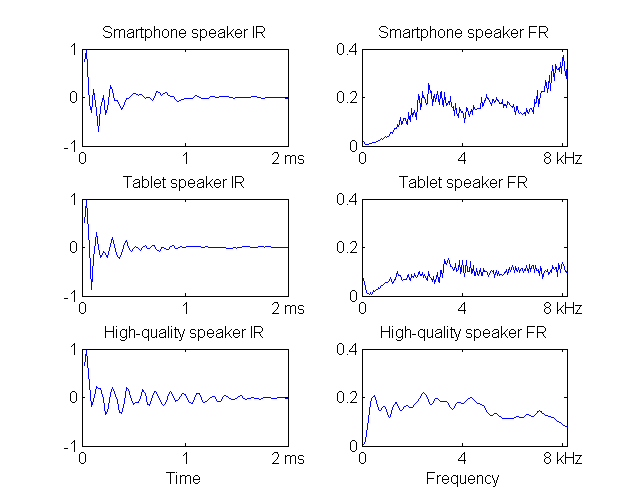
\includegraphics[width=1\linewidth]{Figs/IRs.png}
	\caption{Impulse responses (left) and corresponding frequency transmittance (right) of the three speakers used for playback emulation.}
	\label{fig::IRs}
\end{figure}

When modelling a replay attack one should take into account the impact of the following elements:

\begin{itemize}
\item acoustic effects introduced by the recording device;
\item acoustic conditions in the environment where the voice was acquired;
\item acoustic effects of the replay device, and the
\item acoustic conditions in the environment where the attack takes place. 
\end{itemize}

\begin{figure}
	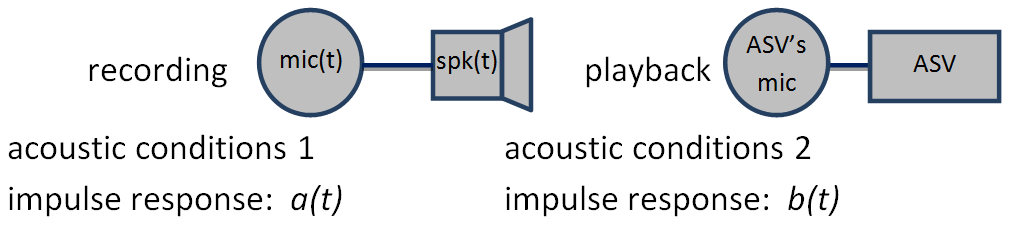
\includegraphics[width=1\linewidth]{Figs/replay.png}

	\caption{Schematic diagram of replay.}
	\label{fig::Replay}
\end{figure}



If $x(t)$ is the speech signal of the client, the playback (spoofing) signal $y(t)$ can be represented by:

\begin{equation}
y(t) = x(t)* mic(t) * a(t) * spk(t) * b(t)
\label{eq::playback}
\end{equation}

where * denotes convolution, $mic(t)$ and $spk(t)$ are impulse responses of the microphone and the speaker, respectively, and $a(t)$ and $b(t)$ are impulse responses of recording and replay environments, respectively (see Fig.~\ref{fig::Replay}). 

Since in this study (as in the majority of other studies on speaker recognition) the NIST databases are used, it implies that the telephony speech will be used. Therefore the $mic(t)$ and $a(t)$ components from the Equation~\ref{eq::playback} are already determined by the source database, and it can be simplified to:

\begin{equation}
y(t) = x(t)* spk(t) * b(t)
\label{eq:playback_simple}
\end{equation}

To emulate replay attacks at the sensor level we need therefore to reproduce the distortions caused by a replay device ($spk(t)$) with and without the effects introduced by acoustic conditions ($b(t)$). We decided to use the following replay devices:

\begin{itemize}
\item a speaker of a popular smartphone brand, from now on in referred to as 'smartphone';
\item a speaker of a popular tablet brand, from now on in referred to as 'tablet';
\item a stand-alone high-quality speaker, from now on in referred to as 'stand-alone speaker'.
\end{itemize}

The impulse responses of these speakers are publicly available~\cite{Brown2014}. Together with frequency responses, they are presented in Fig.~\ref{fig::IRs}.

%\footnote{http://www.aaronbrownsound.com/}.


\begin{figure}
	\centering
	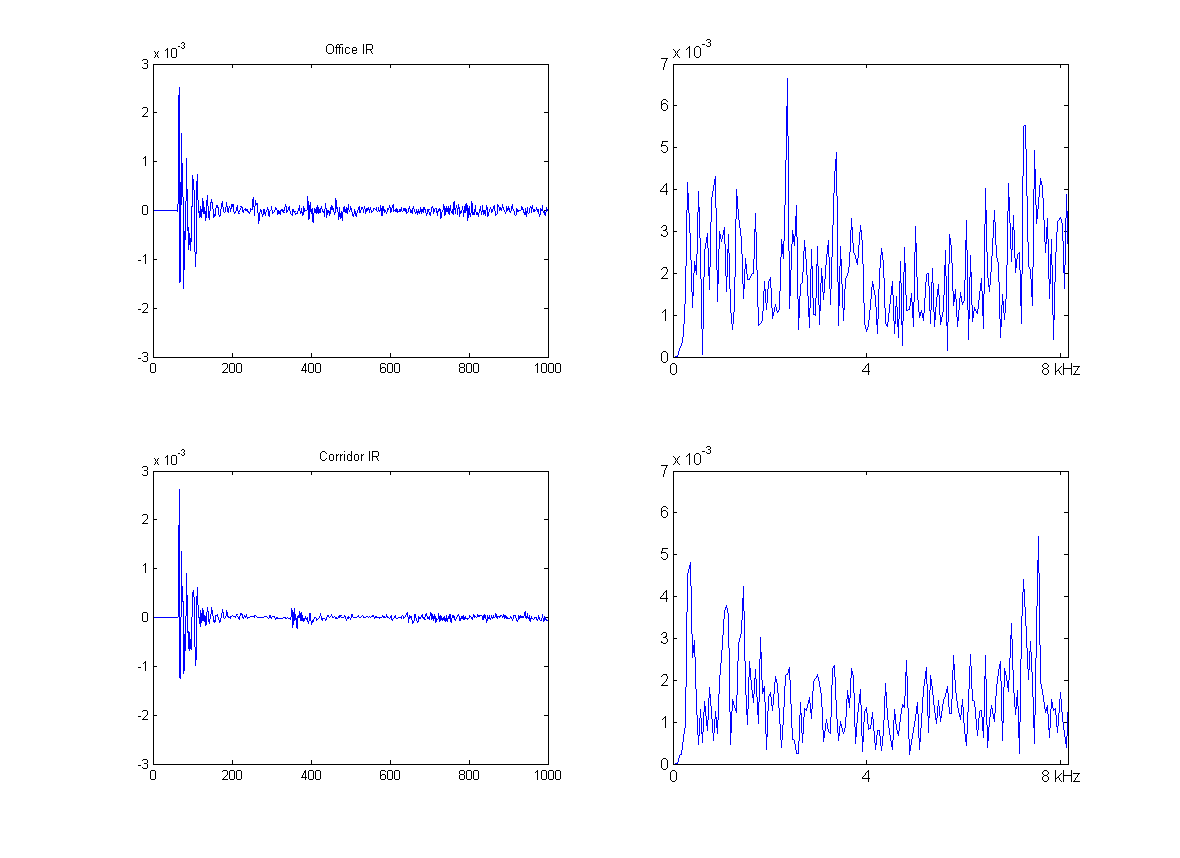
\includegraphics[width=1\linewidth]{Figs/Room_IRs.png}
	\caption{Impulse responses (left) and corresponding frequency transmittance (right) of the office and the corridor used for playback emulation.}
	\label{fig::Room_IRs}
\end{figure}

We decided to emulate two likely environments for a spoofing attack: an office room and a corridor. The corresponding impulse responses were taken from the Aachen Impulse Response (AIR) database ~\cite{Jeub2009}. We used the impulse response of the office room sized 5.00m x 6.40m x 2.90m, with glass windows, concrete walls, a carpet and typical office furniture, and the impulse response of the corridor sized 18.25m x 2.5m x 2.90m, with concrete walls, five wooden doors and one glass door. To check the impact of replay environment we also run experiments without considering the room acoustics, what would correspond to an anechoic chamber.

